% Commuters: who keeps losing (analyze/commute_analysis.py).
\begin{figure}[H]
    \centering
    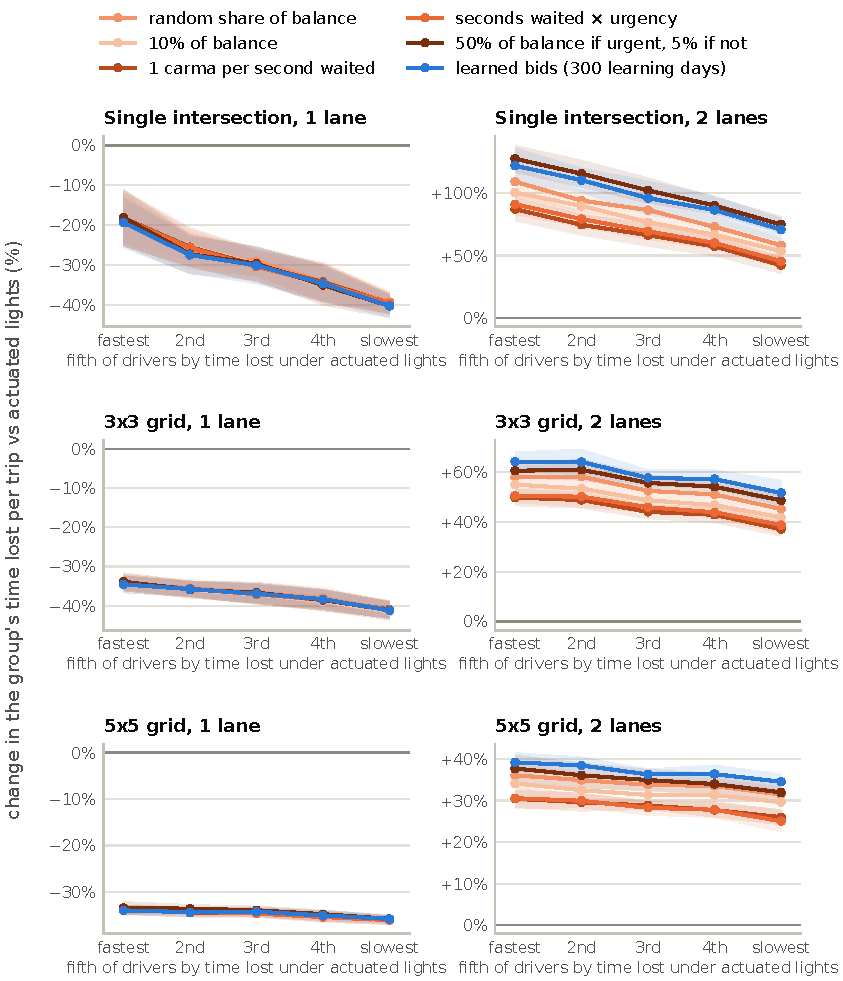
\includegraphics[width=\linewidth]{commute_fifths.pdf}
    \caption{Commuters, who drive the same trips every day: drivers are split into fifths by
    their time lost per trip under actuated lights (evaluation days 1--3), and each fifth's time
    lost under every policy is compared with its time lost under actuated lights on days 4--7. A
    line rising to the right means the drivers who already lose most lose even more; a falling
    line means the policy compensates them. In seconds, at 1 lane the slowest fifth gains about
    twice as much as the fastest; at 2 lanes on the grids every fifth loses a similar number of
    seconds, so the percentage falls. Every driver uses the same rule; fixed rules after
    60 warm-up days, learned bids after 300 learning days; means of 10 seeds, bands 95\%
    intervals; each panel has its own scale.}
    \label{fig:commute_fifths}
\end{figure}

\begin{figure}[H]
    \centering
    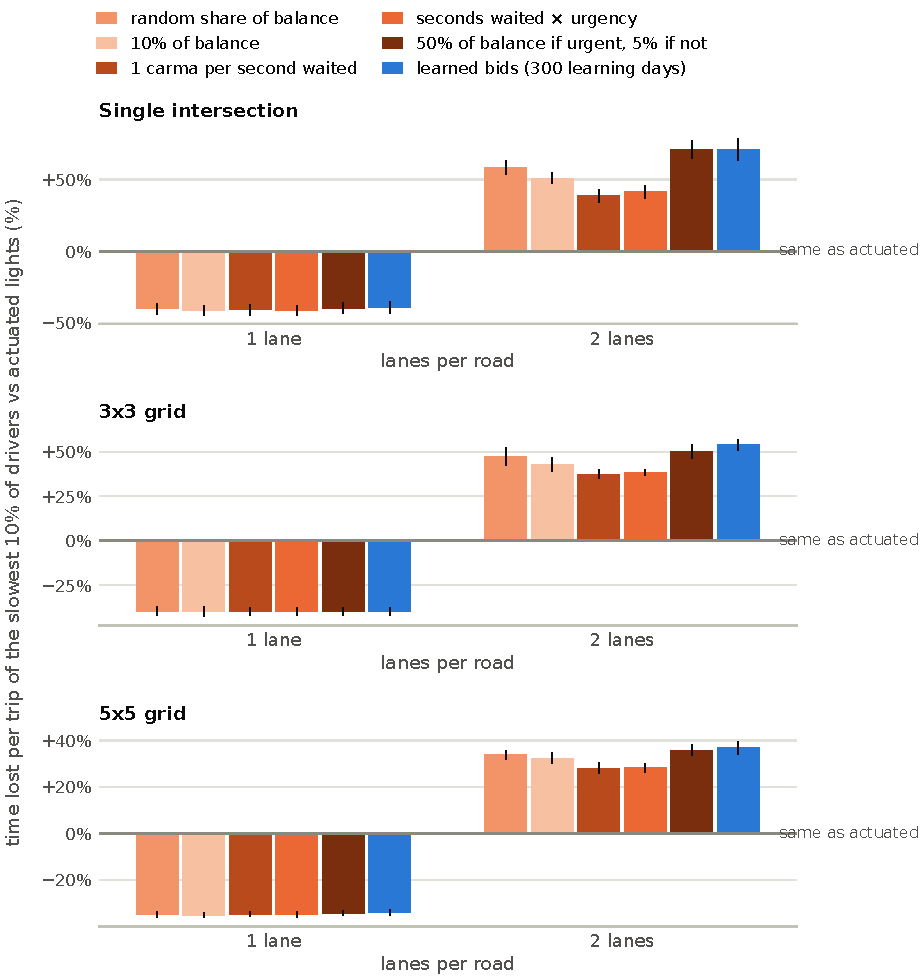
\includegraphics[width=\linewidth]{commute_drivers_tail.pdf}
    \caption{Commuters: average time lost per trip of the slowest 10\% of drivers over the
    evaluation week, compared with the slowest 10\% under actuated lights. Settings as in
    Figure~\ref{fig:commute_fifths}; bars are means of 10 seeds, whiskers 95\%
    intervals.}
    \label{fig:commute_drivers_tail}
\end{figure}
